\section{Introduction}
\label{sec:intro}

We set out to train a multi-turn code agent with RL and could not explain our own training curve.
Over 150 GRPO steps on Qwen2.5-Coder-1.5B, pass@1 on a held-out EvalPlus split rose 2.6--2.8
points across three independent runs (\emph{p} = 0.064 / 0.078 / 0.077 --- none significant at
$\alpha$ = .05; the evidence is the consistent direction across two algorithms and two seeds, not
any single test). But \textbf{91--94\% of newly-passing items passed on the first turn}, and items
rescued by turn 2 or later stayed flat at \textbf{6--9 out of 540} from step 0 to step 150
(Appendix~\ref{app:extra}). The natural reading is that a 1.5B model cannot learn multi-turn
repair. The actual reason is that \textbf{the tool was never successfully called}. Not rarely ---
never. And nothing in the stack said so: the server returned HTTP 200, \texttt{tool\_calls} was an
empty array, and the training loop recorded a well-formed single-turn trajectory.

\begin{figure}[t]
\centering
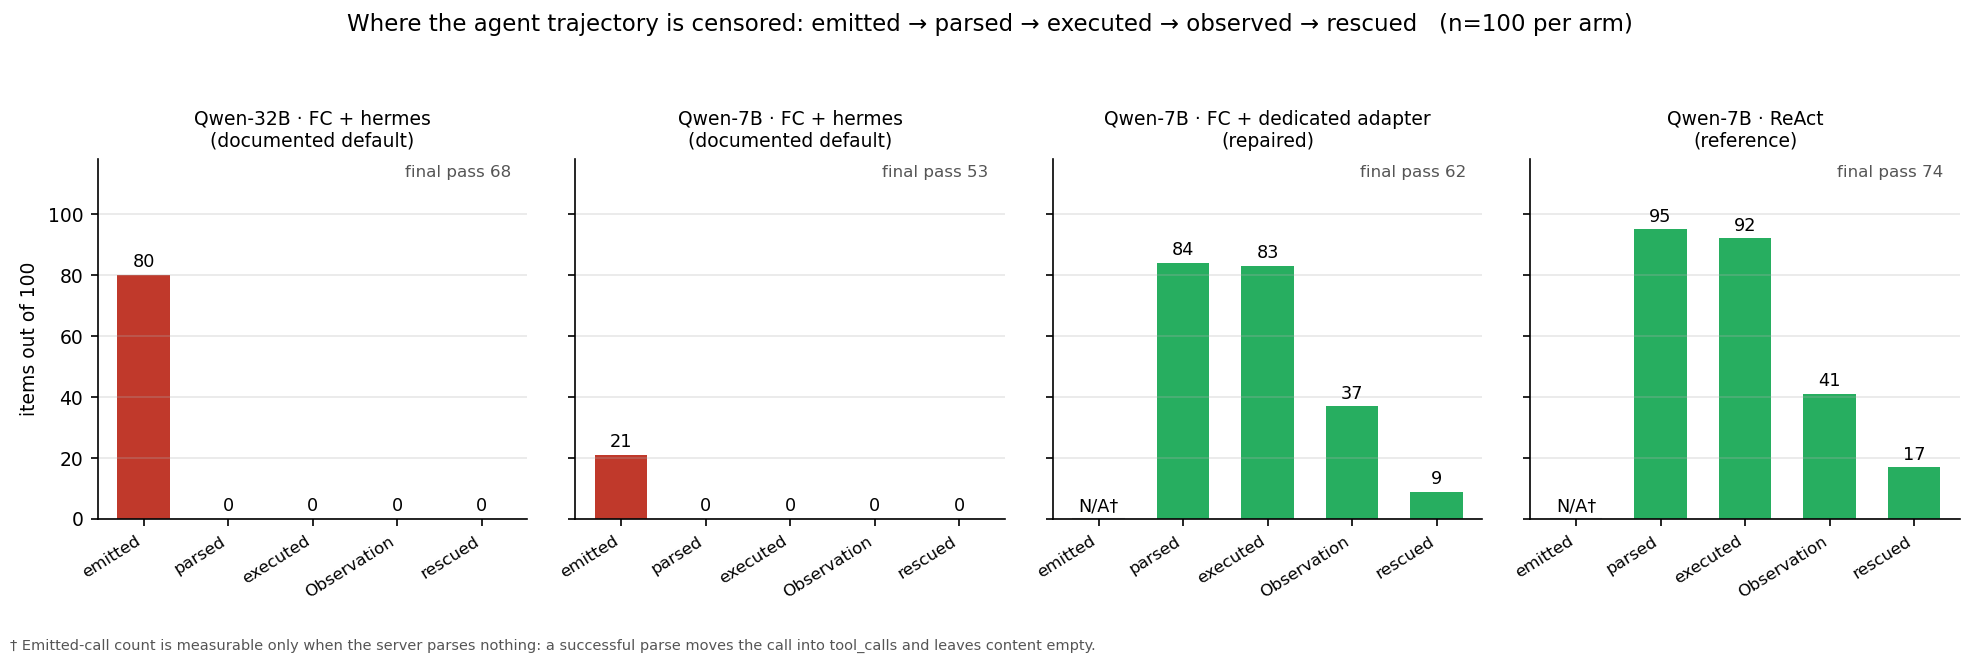
\includegraphics[width=\linewidth]{fig0_funnel.png}
\caption{\textbf{Where the agent trajectory is censored.} Five layers, $n{=}100$ per arm. The two
left panels (documented default configuration) show a tall first bar and a cliff to zero: the
model emits well-formed calls and nothing downstream happens. Emitted-call counts are measurable
only where the server parses nothing --- a successful parse moves the call into
\texttt{tool\_calls} and empties \texttt{content} --- so those cells are N/A, not zero.}
\label{fig:funnel}
\end{figure}

An agent evaluation does not measure a model. It measures a composition
\texttt{model $\times$ protocol $\times$ serialization $\times$ parser $\times$ execution stack},
and the failure of most stages is indistinguishable at the output from model incapability: when a
parser does not recognise the format a model emits, the serving layer reports zero tool calls ---
exactly what a model that refuses to use tools would produce. We call this
\textbf{interface-induced trajectory censoring}.\footnote{\emph{Censoring} is borrowed by analogy.
In survival analysis it is a threshold on a continuous variable; a parser is a deterministic
filter on output \emph{format}. What carries over is the structure of the inference error: the
observation is not missing at random, it is systematically unobservable on one side of a boundary,
and the boundary correlates with the quantity being measured --- positively with checkpoint size,
within this family.} It acts in two opposite directions, and our results contain a clean instance
of each: \textbf{masking}, where a valid call is not recognised and the action never reaches the
environment (Qwen2.5-Coder, \S\ref{sec:scale}), and \textbf{suppression}, where an invalid call is
removed from the sampleable support before it becomes an action (Llama-3.1-8B,
\S\ref{sec:llama}). The correct general statement is therefore neither ``the failure is in the
model'' nor ``the failure is in the interface'':

\begin{quote}
\textbf{The serving interface is simultaneously part of the measurement function and part of the
agent's effective action space.}
\end{quote}

Under RL this is literal. The interface sits between the policy and the environment: whatever the
policy emits must survive serialisation and parsing before it becomes an action that earns a
reward. When nothing tool-intended survives that passage, the experience distribution contains no
tool-mediated trajectory at all.

\paragraph{Why this is not a parser bug.}
The term invites a reading we refuse at the outset. Replaying vLLM's own \texttt{hermes} extractor
line by line over every stored first turn in our archive --- 4254 of them, after removing
byte-identical duplicate files --- we find zero cases in which the server failed to parse a call
its own rules would have accepted (\S\ref{sec:scale}). What fails is the \emph{contract} between
three parties configured independently: what the checkpoint was trained to emit, what the chat
template tells it to emit, and what the parser is defined to accept. Qwen2.5-Coder emits a
well-formed bare call and never the \texttt{<tool\_call>} envelope, so \texttt{hermes} not seeing
it is \emph{correct behaviour}; Qwen2.5-Instruct emits the envelope and then breaks the JSON
inside it. Censoring can occur at any boundary along
\texttt{emission $\to$ serialization $\to$ parse $\to$ execution}, and at every one the observable
is identical: HTTP 200 with an empty \texttt{tool\_calls} array. The claim is therefore not that
parsers are buggy but that \textbf{a tool-call rate is a property of a three-way contract, and is
routinely reported as though it were a property of the model alone.}

\paragraph{What is and is not new.}
That Qwen2.5-Coder does not emit \texttt{hermes}-format tool calls was reported in vLLM issue
\#32926 (2026-01-23) together with a \texttt{<tools>} parser proposal; it was closed as \emph{not
planned} and labelled \emph{stale}, so the trap is still live (\S\ref{sec:related}). What this
paper adds is measurement, decomposition and consequence. We measure the funnel on \emph{two}
standard benchmarks --- BFCL~v4 and $\tau$-bench --- where changing only the serving adapter moves
BFCL's reported score from 0.00 to 0.96 / 0.19 and $\tau$-bench's parsed calls from 0 to 636, and
a $2\times2$ over template and parser finds both main effects exactly zero with the whole effect
in their interaction (\S\ref{sec:bfcl}). We separate \emph{model intent} / \emph{emitted format} /
\emph{server parse} / \emph{actual execution} / \emph{multi-turn rescue} into five independently
measured quantities --- reporting only the third is the standard practice we argue against ---
quantify how much censoring removes across a 21$\times$ scale range, and pair that ladder with a
counterfactual under a \emph{matched} envelope where the silent fraction stays at 0--2 instead of
rising to 80 (\S\ref{sec:scale}). Four families failing at template, parser, schema and token
layers motivate a layered taxonomy, on deliberately asymmetric evidence we mark as such
(\S\ref{sec:families}). And we follow the distortion into training: at 7B, 45 of 115 generations
inside verl's AgentLoop carry a complete call and none becomes an action, so the sampled
experience contains no tool-mediated trajectory to reinforce. We argue that from the sampled
rollouts, not the support of the policy --- \emph{zero observed samples is not zero probability}
--- and the comparison arm changes protocol and interface together; the parser-repair control that
would separate them is a code change blocked by scale, not by the stack (\S\ref{sec:norepair}).
